\subsection*{Problema 24}

\textbf{Enunciado:} Calcular la integral:
\begin{equation*}
\int \dfrac{2x}{(x^2 + x + 1)^2} dx
\end{equation*}

\textbf{Solución:}

Primero, completamos el cuadrado
en el trinomio del denominador:
\begin{align*}
x^2 + x + 1 &= \left(x + \dfrac{1}{2}\right)^2 + \dfrac{3}{4}
\end{align*}

Reescribimos la integral original
con esta nueva expresión:
\begin{align*}
I &= \int \dfrac{2x}{\left(\left(x + \frac{1}{2}\right)^2 + \frac{3}{4}\right)^2} dx
\end{align*}

Aplicamos la sustitución trigonométrica
sugerida:
\begin{align*}
x + \dfrac{1}{2} &= \dfrac{\sqrt{3}}{2}\tan(\theta) \\
dx &= \dfrac{\sqrt{3}}{2}\sec^2(\theta) d\theta
\end{align*}

Además, expresamos $2x$ en función
de $\theta$:
\begin{align*}
2x &= 2\left(\dfrac{\sqrt{3}}{2}\tan(\theta) - \dfrac{1}{2}\right) \\
&= \sqrt{3}\tan(\theta) - 1
\end{align*}

El denominador se transforma como:
\begin{align*}
\left(x + \dfrac{1}{2}\right)^2 + \dfrac{3}{4} &= \dfrac{3}{4}\tan^2(\theta) + \dfrac{3}{4} \\
&= \dfrac{3}{4}\sec^2(\theta)
\end{align*}

Elevando al cuadrado el denominador
anterior:
\begin{align*}
\left(\dfrac{3}{4}\sec^2(\theta)\right)^2 &= \dfrac{9}{16}\sec^4(\theta)
\end{align*}

Sustituimos todo en la integral:
\begin{align*}
I &= \int \dfrac{(\sqrt{3}\tan\theta - 1)}{\frac{9}{16}\sec^4\theta} 
\left(\dfrac{\sqrt{3}}{2}\sec^2\theta\right) d\theta \\
&= \dfrac{8\sqrt{3}}{9} \int \dfrac{\sqrt{3}\tan\theta - 1}{\sec^2\theta} d\theta
\end{align*}

Separamos la integral en dos partes
utilizando identidades trigonométricas:
\begin{align*}
I &= \dfrac{8}{3}\int \sin\theta\cos\theta d\theta \\
&\quad - \dfrac{8\sqrt{3}}{9}\int \cos^2\theta d\theta
\end{align*}

Resolvemos ambas integrales usando
sustitución simple y ángulo doble:
\begin{align*}
I &= \dfrac{4}{3}\sin^2\theta 
- \dfrac{4\sqrt{3}}{9}\left(\theta + \sin\theta\cos\theta\right) + C
\end{align*}

Retornamos a la variable original $x$
empleando el triángulo rectángulo:
\begin{align*}
\sin\theta &= \dfrac{x + \frac{1}{2}}{\sqrt{x^2 + x + 1}}, \quad
\cos\theta = \dfrac{\frac{\sqrt{3}}{2}}{\sqrt{x^2 + x + 1}}
\end{align*}

Sustituyendo los resultados algebraicos
finales, obtenemos la antiderivada:
\begin{align*}
F(x) &= -\dfrac{2x + 1}{3(x^2 + x + 1)} \\
&\quad - \dfrac{4\sqrt{3}}{9}\arctan\left(\dfrac{2x+1}{\sqrt{3}}\right) + C
\end{align*}

\begin{figure}[H]
	\centering
	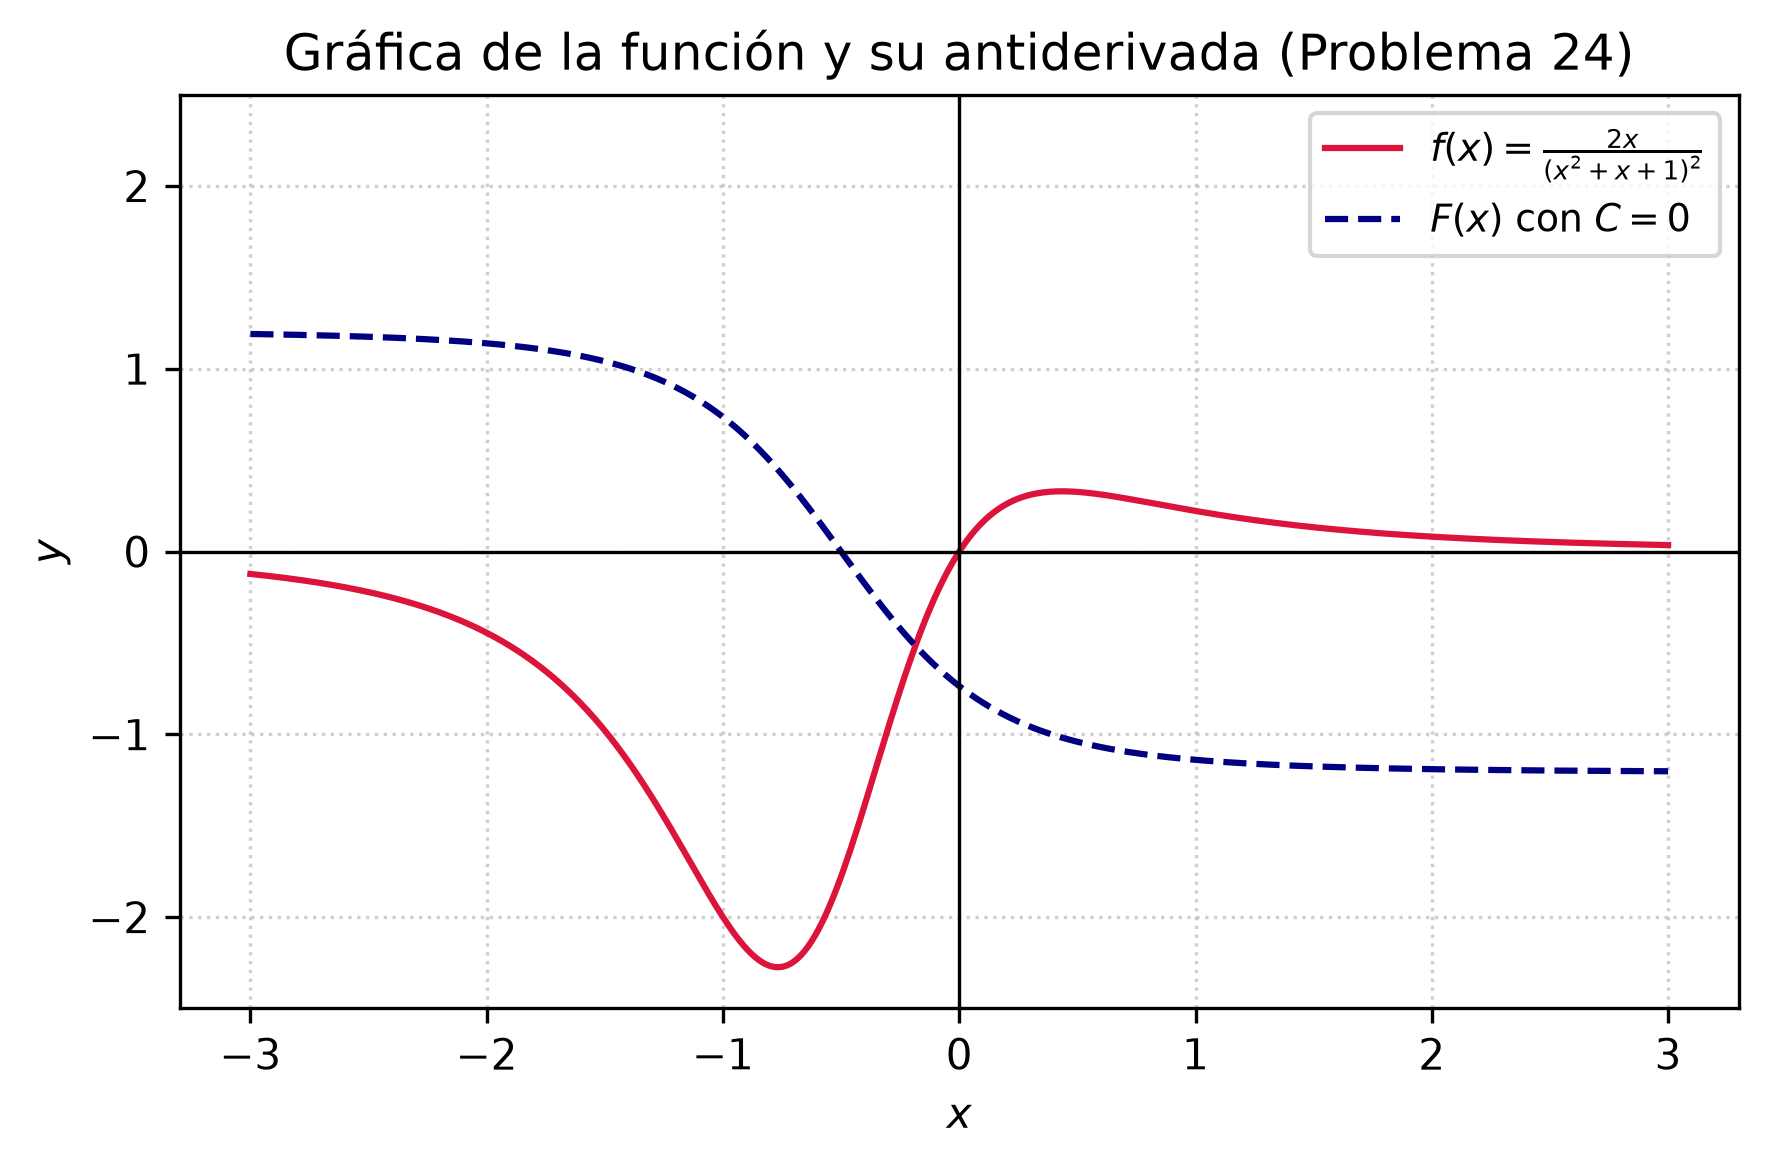
\includegraphics[width=\columnwidth]{semana_03/graficas/SEM03_P24_grafica.png}
	\caption{Representación gráfica de $f(x)$ y su antiderivada $F(x)$ evaluada para la constante de integración $C = 0$ (Problema 24).}
	\label{fig:problema24}
\end{figure}
